\section{Review of \EP{} for energy simulation of building} % we use \EP{} for EnergyPlus to keep consistency

In this section, we review the \EP{} software program, which provide
accurate input and output traces from buildings for the new thermal
modeling algorithm.

The \EP{} software package ~\cite{energyplus:2001vf} is a suite of
algorithms that calculate the energy required to operate a building
and its resulting thermal behavior based on numerous considerations
ranging from the specifications of the structure, to heat sources and
sinks within the building, and weather.
% Whole building performance tool is utilized to design energy efficient
% building. DOE-2 used to be one of the most popular programs used for
% designing energy efficient building.  It was develop and released in
% the late 1970s and early 1980s. DOE-2 was written in older version of
% Fortran and this will be a problem for the new compilers. \EP{} is
% developed by the U.S. Department of Energy based on DOE-2 and add more
% features.
\EP{} consists of  an integrated solution
manager that manages the calculation of the heat balance of various
surfaces in the building, the heat balance of the air, and the heat
balance on the mechanical systems. The solution to each of these three
elements is calculated separately and communicated to each other
using the manager at each time-step.
% \EP{} is a well-organized, module-concept comprehensive
% whole building performance simulation tool.
Due to its modularity, it is easy to establish links to other programs such as Google SketchUp for 3D building display.
% and \EP{} can deal with more complex system and
% generate more accurate results than DOE-2. It is used to model the
% energy using in the building, such as heating, cooling, lighting and
% other energy flows.

An input data file (IDF) and weather file are needed for the \EP{}
simulation. The IDF includes all the information of the building such
as size, structure, position and the HVAC subsystem, etc. The IDF
editor in \EP{} can be used to change parameters of the building, the
schedule of the HVAC subsystem and also the output information. The
selected output information is generated in the spreadsheet file
after running the simulation.

Fig.~\ref{fig:5zone} shows the side view and the top view of an office building
with 5 rooms and HVAC modeled in \EP{}.  The heat sources for this building
can be HVAC, light, occupants, electric equipment, air filtration, etc. The
room temperature is also affected by the weather (ambient temperature and solar
effects) and can be controlled by the HVAC system with coil
and fan.

%  as shown in
% Fig.~\ref{fig:coil-fan-diagram}.
% The air of a room are cooled or
% heated in the coil and goes back to the zone. The coil itself is a
% heat exchanger. Besides the air loop, the coil has a water loop coming
% from the boiler or chiller to control the temperature of the air.

% Fig.~\ref{fig:energyplus-graph} shows the simulated temperature
% changes over 500 hours in the 5 zones (rooms) from this building form
% \EP.

\begin{figure}[t]
    \centering
    \subfloat[]{
        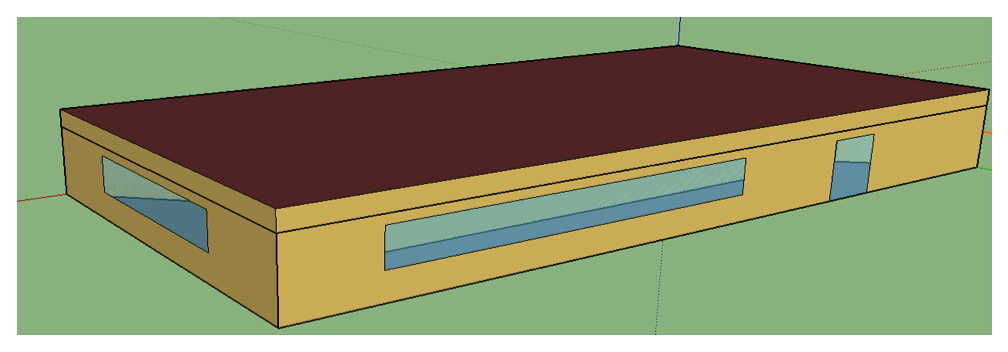
\includegraphics[width=0.539\columnwidth]{figs/energyplus_review/5zone-a}
    }
    \subfloat[]{
        \includegraphics[width=0.361\columnwidth]{figs/energyplus_review/5zone-b}
    }
    \caption{The 5-zone office building (a) side view (b) top view.}
    \label{fig:5zone}
\end{figure}

Fig.~\ref{fig:energyplus-io-curve} shows the simulated temperature changes and
input changes over 15 days from \EP{} for an office building with the 5 zones
(rooms), as shown in Fig.~\ref{fig:5zone}.  \EP{} can assign different schedules
for each room while simulating the thermal model.
Fig.~\ref{fig:occupancy-curve} shows a typical working schedule of the 5 rooms
of the office building.

\begin{figure}[t]
    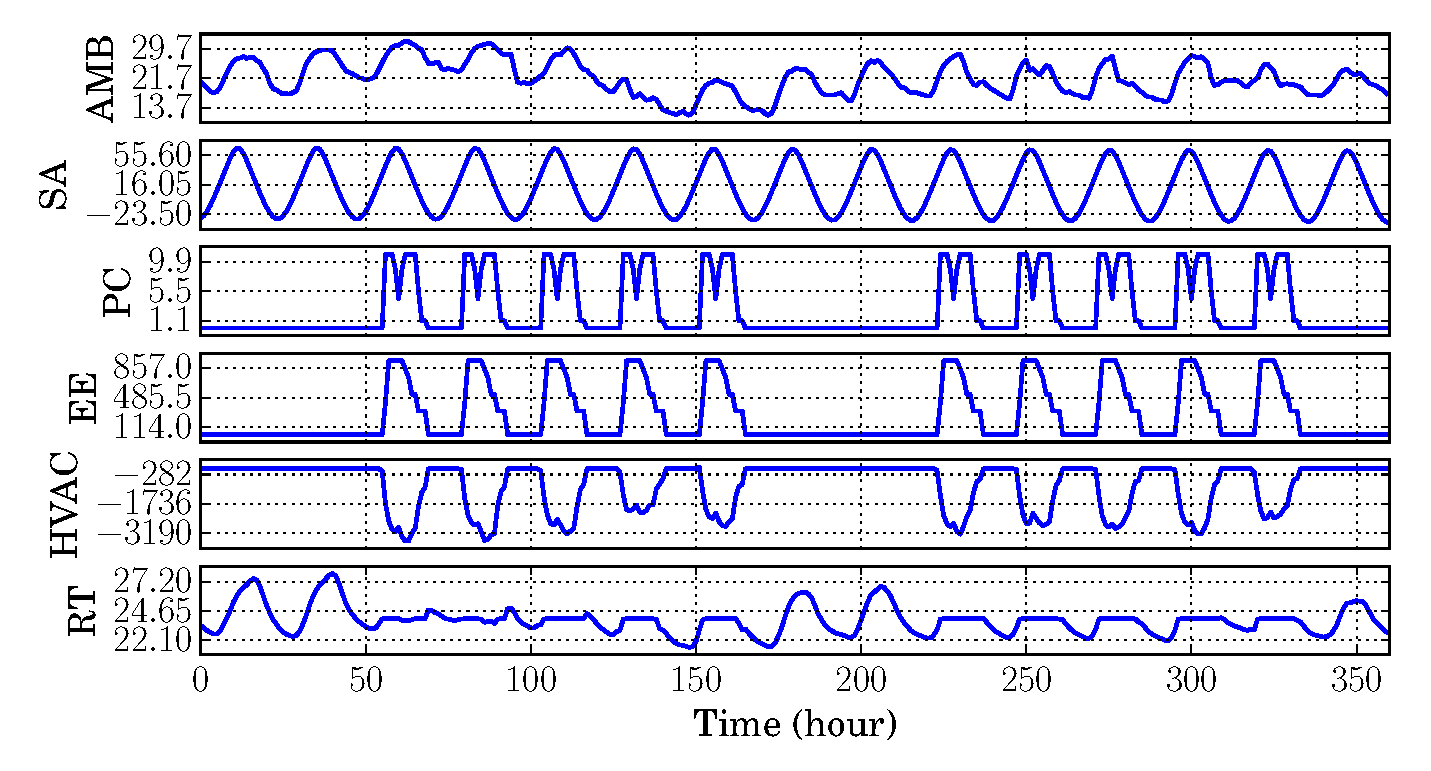
\includegraphics[width=0.9\columnwidth]{figs/energyplus_review/energyplus}
    \caption{Selected \EP{} input and simulated temperature output data sample in
        15 days.  (AMB: AMBient temperature; SA: Solar Angle; PC: People Count
        (occupancy); EE: Electrical Equipment power; HVAC: HVAC system
        cooling/heating power; RT: Room Temperature)}
    \label{fig:energyplus-io-curve}
\end{figure}
\begin{figure}[t]
\centering
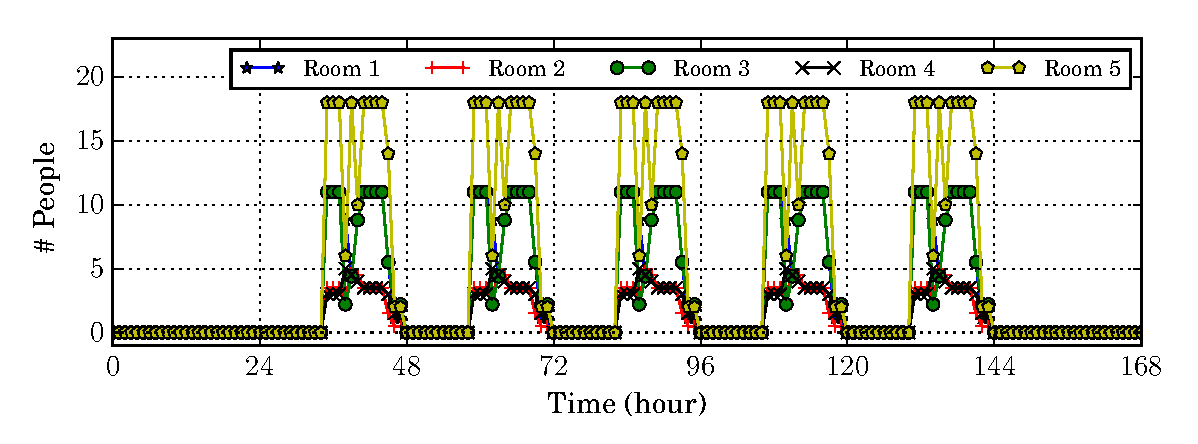
\includegraphics[width=0.9\columnwidth]{figs/energyplus_review/occupancy}
\caption{Occupancy information of 5 rooms during one week.}
\label{fig:occupancy-curve}
\end{figure}

%
%In this particular example, we have many inputs for each output, which
%is the temperature of each zone (room). Selected inputs are shown in
%Fig.~\ref{fig:energyplus-io-curve}. The main heating sources comes
%from information technology equipment (ITE) as this is a date center
%building.  ITE is a group of equipment such as computers, monitors,
%servers, printers, network hubs etc. With the increasing of computing
%capacity in the data center, ITE becomes a significant power consumer
%and the cooling of ITE is required. Inputs 5 and 6 comes from HVAC
%for the cooling. Notice that ambient temperature is also input for
%our thermal model.

We want to stress that fundamentally thermal behavior of building
systems is typically nonlinear (at least weakly nonlinear) due to the
temperature-dependent properties of the building materials and thermal
radiation effects. As a
result, nonlinear modeling is preferred for accurate temperature
control and management.

